\documentclass[twocolumn]{article}
\usepackage[utf8]{inputenc}
\usepackage[top=1in]{geometry}
\usepackage{graphicx}
\usepackage{hyperref}
\input{sym}
\title{ECE 417/598: Homework 1}
\author{Max marks: 120}
\date{Due on Jan 28, 2021, before class.}
\newtheorem{prob}{Problem}

\newcommand{\bx}{\bar{x}}
\newcommand{\by}{\bar{y}}
\newcommand{\bz}{\bar{z}}
\begin{document}

\maketitle
\section{Jan 24 Lecture}
\begin{prob}
  For the given robot write down the axis-angle rotation from joint to joint
  assuming the joint angles to be  $\theta_1$, $\theta_2$, $\theta_3$ respectively.
  \\
  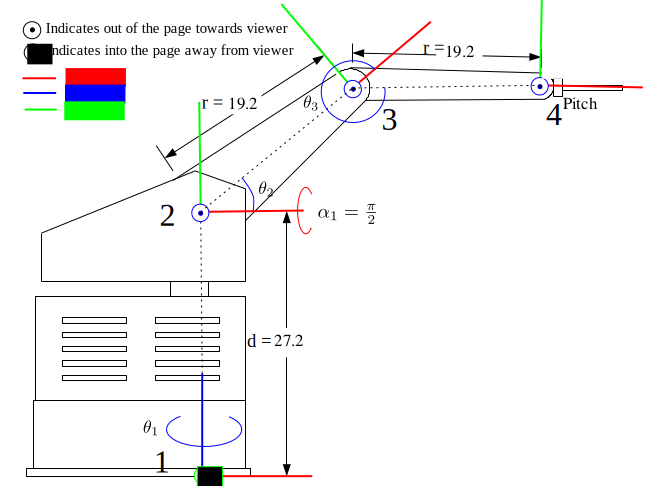
\includegraphics[width=\linewidth]{robot.png}
  \\
\end{prob}

\section{Jan 26 Lecture}
\begin{prob}
  The following is known about a smooth trajectory: p(0) = 0, v(0) = 0, 
  p(3) = 2, p(7) = 0, v(7) = 0 and velocity and acceleration are 
  continuous everywhere.  

  \begin{enumerate}
  \item What is the lowest degree single polynomial which could be used?  
  \item Give two advantages to using a spline curve instead. 
  \item What degree polynomials would you suggest for the splines?  
  \item Write the polynomials.  
  \item Write the set of equations which would be used to solve for the coefficients. Do not use normalized time. 
  \item Solve for the coefficients.
  \item Write the set of equations which would be used to solve for the coefficients. Use normalized time. 
  \item Solve for the coefficients.
  \end{enumerate}
\end{prob}


%\bibliography{main}
%\bibliographystyle{plain}
\end{document}